\chapter{Title of this chapter}
\label{chapter:something}


Abstract of chapter 1

\section{Introduction}


\section{Objectives}
\label{section:ch03:objectives}

This chapter addresses the following objective of the thesis:

\begin{itemize}
    \item \textit{\Paste{objtwo}}

\end{itemize}


This chapter also covers the following research question:

\begin{itemize}
    \item \textit{\Paste{rqtwo}}
\end{itemize}

This question is answered based on ....

\section{Methods}

\begin{figure}[H]
\centering
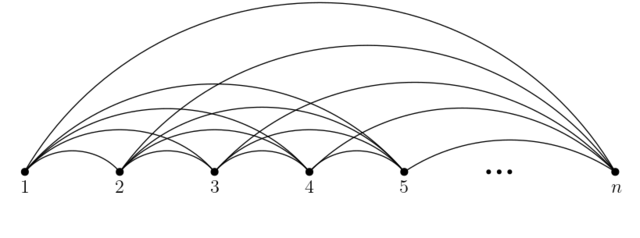
\includegraphics[width=\textwidth]{figures/sample_graph.png}
\caption{Figure caption goes here}

\end{figure}

Example code excerpt
\begin{lstlisting} 
Name.prototype = {
  methodName: function(params){
    var doubleQuoteString = "some text";
    var singleQuoteString = 'some more text';
    // this is a comment
    if(this.confirmed != null && typeof(this.confirmed) == Boolean){
      document.createElement('h3');
      $('#system').append("This looks great");
      return false;
    } else {
      throw new Error;
    }
  }
}
\end{lstlisting}

